\section{Vertexing}
\label{sec:vertexing}

\subsection{General problem formulation}

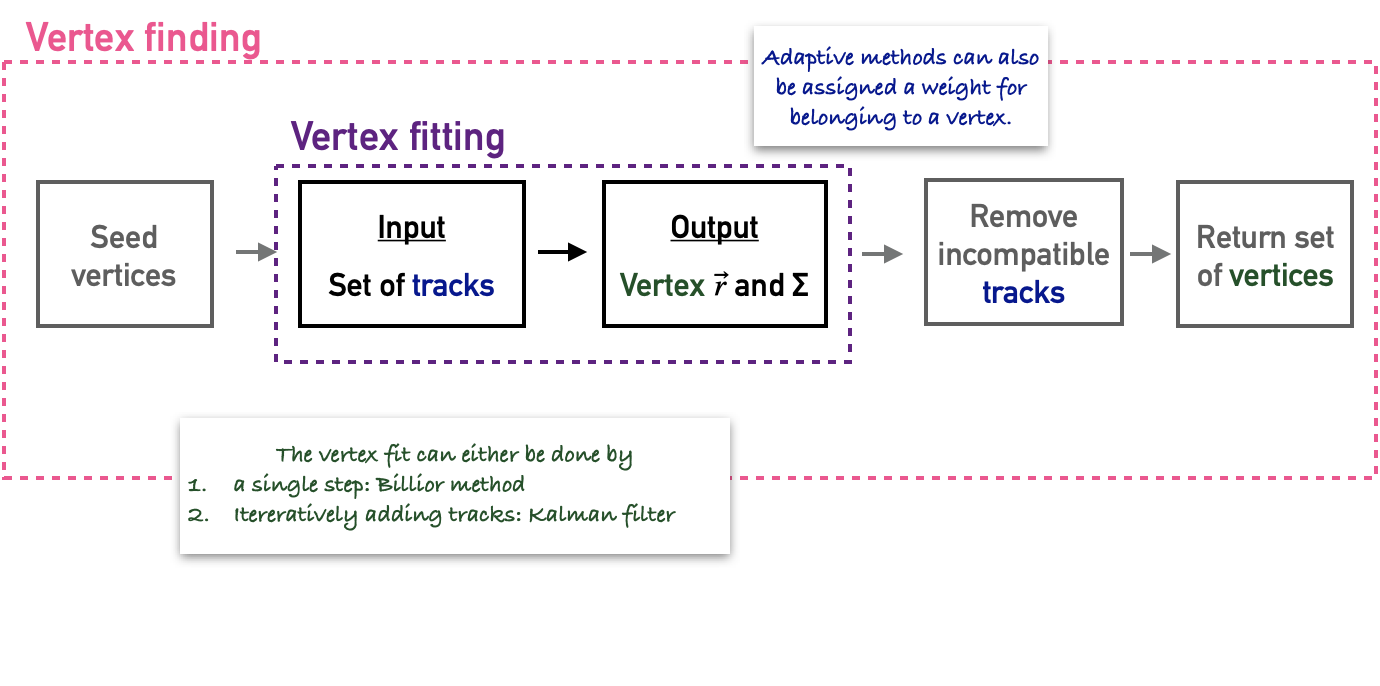
\includegraphics[width=\textwidth]{figures/cp-graphics/Vertex-finding-fitting}

The \textcolor{rebeccapurple}{Vertex fit:} Position which maximizes the likelihood for the probability density tubes for the tracks to all intersect at this point \cite{giacinto-thesis}. 
This is seen mathematically by \Eq{\ref{eq:vtx-prob-density-fct}} below, where $\vec{r}$ is the position of the vertex, and $\vec{r}_i(\phi_{p,i})$ is track $i$ and $\phi_{p,i}$ parametrizes what point of the trajectory that we're on.

\begin{equation}
P(\vec{r}) = \int d \phi_{p,1} d \phi_{p,2} \ldots d \phi_{p,n} \prod_{i=1}^{n_{trk}} 
\exp \left[ - \frac{1}{2}  \left(\vec{r} - \vec{r}_i (\phi_{i,i})\right)^T COV^{-1}_{3x3} (\phi_{p,i}) \left(\vec{r} - \vec{r}_i (\phi_{i,i})\right) \right]
\label{eq:vtx-prob-density-fct}
\end{equation}

\hl{Is this cov matrix the vertex cov? If so, should I call it $\Sigma$ instead of $Cov_{3x3}$?}

\subsection{Primary vertex reconstruction}

The event's selected primary vertex (PV) is defined as the reconstructed primary vertex with largest $\sum \pT^2$ of the associated tracks. 
